\graphicspath{{capitulos/Capitulo4-Implementacion/recursos/}}

\section{Implementación} \label{capitulo:4}

Como ingeniero informático, este proyecto se ha desarrollado de forma orientada al proceso de ingeniería de software que consta de las siguientes etapas o procesos: 
\begin{enumerate}
    \item Planificación
    \item Análisis
    \item Diseño
    \item Implementación propiamente dicha
    \item Pruebas
    \item Despliegue y explotación    
\end{enumerate}
%planificación, análisis, diseño, implementación propiamente dicha, pruebas y despliegue/explotación. 
Adicionalmente existe la etapa de monitorización y seguimiento que se desarrollan posteriormente de la puesta en marcha del sistema en un entorno real, y esto no forma parte del presente TFM debido a su naturaleza de investigación (al igual que el propio máster), así que no se han llevado a cabo dichos procesos.

En las sucesivas secciones de este capítulo iremos describiendo los procesos llevados a cabo en cada una de estas etapas y las conclusiones alcanzadas en las mismas.

\subsection{Planificación}
\label{sec:4:planificacion}
En esta primera etapa presente en todo proyecto tratamos de fijar principalmente el concepto de alcance, que podríamos definir como el trabajo realizado para entregar un producto, servicio o resultado con
las funciones y características especificadas~\cite{PMBOK}.

Los proyectos de naturaleza de investigación e innovación como éste requieren de una cierta flexibilidad a la hora de definir el alcance, puesto que planteamos hipótesis iniciales que en función de ser válidas o no, plantearemos otras nuevas. Como éste TFM forma parte de un proyecto mayor, es más sencillo definir el alcance, aunque este sufrió alguna modificación.

El proyecto parte con la definición de las hipótesis iniciales recogidas en la \autoref{sec:Hipotesis}. 
Pretendía abarcar en primera instancia la comprensión del dominio del problema y la lógica de negocio sobre la que poder comenzar a trabajar, y tras ello, podría dar comienzo el desarrollo de la metaheurística VNS descrita en el \autoref{capitulo:3} y analizar los resultados comparándolos con el SA (experimentación, recopilado en el \autoref{capitulo:5}). Al comienzo del proyecto se implementarían los 5 tipos de VNS descritos previamente:
\begin{itemize}
	\item Variable Neighborhood Descent (VND)
	\item Reduced Variable Neighborhood Search (RVNS)
	\item Basic Variable Neighborhood Search (BVNS)
	\item General Variable Neighborhood Search (GVNS)
	\item Skewed Variable Neighborhood Search (SVNS)
\end{itemize}

Y posteriormente fue ampliado con la variación de la naturaleza de los entornos probabilista.

Por otro lado, el sistema organizativo acordado con los tutores para este TFM consistió en un desarrollo iterativo en ciclos marcados por metas en una jornada de trabajo en un despacho ofrecido por el grupo de investigación de 8 horas diarias de Febrero de 2019 a Junio de 2019. Finalmente las fechas fueron ampliadas. Se trata de una variación de los sprints de SCRUM combinada con un tablero KANBAN creado en la aplicación web Tello. 

A continuación describiremos cada uno de esos ciclos.

El primer ciclo incluía el proceso de planificación y de análisis junto al estudio del sistema y los documentos previos facilitados por los tutores (\textit{literature review}). Tuvo por meta la comprensión del dominio del problema (primera parte) y de la lógica de negocio utilizada en los antecedentes del TFM (véase la \autoref{capitulo:2:detalles-sistema})

Los demás ciclos únicamente requerirán de las fases de diseño, implementación y pruebas. La meta para el segundo era la implementación de la \faseuno{} (diseño, implementación y pruebas). El tercer ciclo como meta fue la implementación de una primera versión funcional del sistema implementando unicamente el VND, definiendo previamente los diferentes entornos a emplear. Para el cuarto ciclo se debían implementar el resto de variaciones del VNS así como realizar un despliegue del sistema empaquetandolo y enviandolo en forma de entrgable a los tutores (véase la \autoref{sec:4:despliegue}). El cuarto ciclo fue añadido posteriormente para subsanar errores e implementar los entornos probabilísticos que ya fueron descritos en la \autoref{capitulo:3:busqueda-divers-intens}. Finalmente se encuentra el ciclo de experimentación, donde comparamos los resultados y analizamos la eficiencia del sistema.

En la \autoref{sec:4:implementacion} se describen las tecnologías software utilizadas. %TODO: hacerlo efectivamente

% TODO: ¿cronograma?

\subsection{Análisis}
El objetivo de esta fase consiste en la educción de los requisitos que precisa el software a partir de los documentos e información facilitada por los tutores y demás stakeholders.

Los \textit{stakeholders} del proyecto son: CRIDA, los tutores, y los estudiantes de doctorado o máster implicados actual o anteriormente (Tino Tello, Jónatan Lara y Pablo Lozano) y será a quienes se deberá recurrir para responder dudas. El \textit{stakeholder} principal por supuesto es CRIDA, que guiará los objetivos principales y responderá a las preguntas de mayor complejidad y que competan a dominio del problema. Los tutores tendrán las mismas competencias pero a nivel del TFM y no del proyecto en su totalidad, y serán quienes faciliten la documentación inicial relativa al dominio del problema. El resto de \textit{stakeholders} y especialmente Tino Tello, proporcionarán la información relativa al software y aclararán conceptos de esta índole.

La documentación inicial facilitada por los tutores se basa en dos papers uno publicado y otro sin publicar a fecha de inicio del TFM~\cite{articulo1, articulo2}. Una vez leída la documentación inicial y comprendido el dominio del problema, se realizó una entrevista con Tino Tello para comprender la implementación del sistema \legacy{} para poder comenzar a trabajar. En dicha entrevista se obtuvo como conclusión la creación de un repositorio con control de versiones Git disponible para todos los \textit{stakeholders} y el inicio del primer ciclo de la planificación (definidos en \autoref{sec:4:planificacion}).

En este punto se identifican los requisitos del sistema tanto del dominio (obtenidos del software \legacy{} y de la documentación inicial) como del sistema (entrada/salida, interfaces, etc.) que se encuentran recopilados en las próximas secciones.

\subsubsection{Requisitos del dominio}
\label{sec:4:RD}

Los requisitos de dominio son aquellas restricciones del sistema que son impuestas únicamente por el dominio del problema, y no por la propia naturaleza del sistema ni de forma externa.

Este tipo de requisitos son necesarios para la constitución de una solución factible y permite cuantificar lo mejor o peor que son una solución de otra mediante el conteo (ponderado) del numero de restricciones incumplidas (véase el objetivo \ref{O2}). 

En el sistema \legacy{} existían dos tipos de restricciones: obligatorias y deseables, pues una vez alcanzada la factibilidad se intentaba mejorar. Sin embargo, en este sistema nos moveremos por soluciones infactibles buscando la que sea mejor, a ser posible factible pero no como condición necesaria. Estas restricciones son impuestas por la legislación española, recogidas en el BOE, fundamentalmente en:

\begin{itemize}
	\item Real Decreto 1001/2010, de 5 de agosto, por el que se establecen normas de seguridad aeronáutica en relación con los tiempos de actividad y los requisitos de descanso de los controladores civiles de tránsito aéreo. \\
	(\url{https://www.boe.es/eli/es/rd/2010/08/05/1001/con})
	
	\item Ley 9/2010, de 14 de abril, por la que se regula la prestación de servicios de tránsito aéreo, se establecen las obligaciones de los proveedores civiles de dichos servicios y se fijan determinadas condiciones laborales para los controladores civiles de tránsito aéreo. \\
	(\url{https://www.boe.es/eli/es/l/2010/04/14/9})
\end{itemize} 



En primer lugar tenemos las fundamentales:

%\begin{enumerate}[label={\textbf{RDF\arabic*}}]
\begin{enumerate}[label={\textbf{RD\arabic*}}, ref={RD\arabic*},  align=left]
	
	\item Todas las posiciones de control deben estar cubiertas por controladores de manera exclusiva, exhaustiva y bajo las restricciones definidas.
	\begin{enumerate}[label*={\textbf{.\arabic*}}]
		\item Cada sector y posición, deben ser cubiertos en los intervalos donde estén abiertos (exhaustividad).
		\item Cada sector y posición, deben ser cubiertos por un único controlador (exclusividad).
	\end{enumerate}
	
	\item Un controlador no puede tener dos asignaciones diferentes en el mismo instante.
	\begin{enumerate}[label*={\textbf{.\arabic*}}]
		\item Entendemos por asignación la combinación de sector y posición.
		\item un controlador no puede estar cubriendo en el mismo
		instante la posición de ejecutivo y planificador de un sector y tampoco puede estar
		asignado a dos sectores diferentes en el mismo instante, sea cual sea la posición.
	\end{enumerate}

	\item \label{RD:tipos-sector}  Cada sector tendrá un tipo de sector, que podrá ser Aproximación o Ruta

	\item  \label{RD:sector-nucleo} Cada sector tendrá uno o varios núcleos asociados, así como cada núcleo tendrá un conjunto de sectores (relación N a N)
	
	\item \label{RD:nucleo-controlador} Cada controlador estará acreditado para controlar un único núcleo.

\end{enumerate}



A continuación las relativas a la posición y asignación de los controladores:

\begin{enumerate}[resume*]
	\item \label{RD:acreditacion-valida} Una determinada posición podrá ser asignada a un controlador si el controlador está habilitado en el núcleo al que pertenece el sector que le corresponde, o bien en uno de los núcleos a los que pertenece el sector
	(si este es un sector común) independientemente de la sectorización por la que el sector se encuentre abierto.
	
	\item A un controlador tipo CON solo podrá asignársele una posición cuyo sector sea Ruta (véase la \autoref{table:2:acreditaciones})
	
	\item Los sectores o agrupaciones de dos sectores que se indique en la entrada del problema, se deberán cubrir con 4 controladores en el turno	de noche.

	\item Un controlador solo puede operar en su turno correspondiente: si pertenece al turno largo, en el turno largo y si pertenece al turno corto en el turno corto.

	\item Un controlador no puede cambiar de posición de control de una posición ejecutiva de un determinado sector a una posición ejecutiva de otro sector diferente, sin que exista un descanso entre medias, a no ser que ambos sectores sean afines (cambio de configuración). Nota: si no hay cambio de configuración de sectores no es posible que dos sectores diferentes posean volúmenes comunes.
	
	\item El número máximo de sectores por los que rota un controlador es 3.	
\end{enumerate}



Y por último las relativas a los tiempos de trabajo y descanso de los controladores:

\begin{enumerate}[resume*]
	
	\item \label{RD:porcentaje-min-descanso} El porcentaje de tiempo de descanso mínimo en turno diurno (mañana o tarde), incluyendo turnos largos es del 25\% como mínimo.
	\begin{enumerate}[label*={\textbf{.\arabic*}}]
		\item En caso de los turnos de noche, el porcentaje de tiempo de descanso mínimo en el turno de noche será
	como mínimo del 33 \%.
	\end{enumerate}
	
	\item No es posible un periodo de trabajo continuo mayor de dos horas en los que el controlador no realice ningún periodo de descanso.
	
	\item No puede existir ningún periodo de dos horas y media en los que un controlador realice un periodo total de descanso menor de media hora. Es decir, dentro de una ventana de tiempo de dos horas y media un controlador debe tener mínimo 30 minutos de descanso, sin ser necesario que estos se realicen de forma continua.
	
	\item El tiempo mínimo de trabajo continuado es de 15 minutos.
	
	\item El tiempo mínimo de descanso continuado es de 15 minutos.
	
	\item El tiempo mínimo en posición de un controlador es de 15 minutos.
	
	\item Todos los controladores deben trabajar como mínimo 15 minutos.
		
\end{enumerate}


\subsubsection{Requisitos de entrada/salida}
Los requisitos de entrada y salida (I/O) son aquellos relativos a la los ficheros y formatos definidos tanto para la entrada al sistema como en la salida.

\begin{enumerate}[label={\textbf{RIO\arabic*}}, ref={RIO\arabic*},  align=left]
	
	\item  Una entrada al sistema se compondrá de dos partes: la información de la dependencia y la información del caso, de esta forma, la información común a varios casos será independiente de cada caso concreto.
	
	\item Adicionalmente se empleará un fichero de propiedades que permita modificar los parámetros del sistema (véase lista parámetros del sistema) %TODO: referencia!!!
	sin necesidad de recompilar todo el código.	
	
	\item La información de la dependencia será un subdirectorio con el nombre de la dependencia, contendrá 4 ficheros:
	\begin{enumerate}[label*={\textbf{.\arabic*}}]
		\item  Relación de todos los sectores pertenecientes la unidad de control con los sectores elementales\footnote{
			Sector que comprende una zona del espacio aéreo que no es subdivisible empleando otros sectores. Recuérdese el sector LECMBDP (azul) de la \autoref{fig:2:sectorizacion-3d} se podía sustituir por otros más pequeños, por lo tanto no es elemental
		} por los que están formados cada uno de los sectores.
		\begin{enumerate}[label*={\textbf{.\arabic*}}]
			\item Tendrá las siguientes columnas: Nombre sector (p. ej. LECBBAS) y sector elemental
			\item En caso de ser elemental, la segunda columna deberá ser vacía
		\end{enumerate}

		\item  Matriz de Afinidad de los sectores de la dependencia (definida en la \autoref{section:2:sectores-y-sectorizacion}).
		\begin{enumerate}[label*={\textbf{.\arabic*}}]
			\item Será una matriz cuadrada cuyas filas y columnas son los sectores de la Unidad de Control concreta
			\item Un elemento concreto de la matriz tendrá dos posibles valores:
			\begin{enumerate}[label*={\textbf{.\arabic*}}]
				\item 1 si son afines el sector de la fila con el de la columna.
				\item 0 en caso contrario, es decir, si no son afines entre sí.
			\end{enumerate}
			\item Nótese que todo sector es afín consigo mismo.
		\end{enumerate}
	
		\item Lista de los sectores pertenecientes a la Unidad de Control, en la que se indica el tipo de sector (véase~\ref{RD:tipos-sector}) y los núcleos a los que pertenece (ver~\ref{RD:sector-nucleo}).
		\begin{enumerate}[label*={\textbf{.\arabic*}}]
			\item Tendrá las siguientes columnas: 
			\begin{enumerate}[label*={\textbf{.\arabic*}}]
				\item Nombre sector (p. ej. LECBBAS) 
				\item Tipo Sector. Posibles valores APP o RUTA
				\item Número variable de columnas que representen los núcleos que tiene la dependencia concreta (p. ej. Barcelona TMA, Barcelona Ruta Este y Barcelona Ruta Oeste)
				\item Cada fila tendrá el caracter x en caso de que pertenezca al núcleo
				\item Cada fila podrá tener varias columnas de núcleo marcadas (véase el requisito~\ref{RD:sector-nucleo}).
			\end{enumerate}
		\end{enumerate}
		\item Lista de sectorizaciones de la Unidad de Control y sectores que conforman la sectorización y los volúmenes a los que pertenece cada sector.
		\begin{enumerate}[label*={\textbf{.\arabic*}}]
			\item Tendrá como columnas: la sectorización (2B, 1A,...), el nombre del sector, el volumen al que pertenece y el núcleo al que pertenece.
			\item Debido que cada volumen puede abarcar varios sectores, el nombre del sector y la sectorización se repetirán en varias filas pero cambiando el valor del volumen.
		\end{enumerate}
	\end{enumerate}
	
	\item La información del caso concreto está desglosada en 6 ficheros, dos de ellos opcionales.
	\begin{enumerate}[label*={\textbf{.\arabic*}}]
		\item Definición del turno. Contiene la hora de inicio y fin del turno completo así como del tipo (mañana, tarde, noche y largo o corto).
		\item \label{RIO:apertura-sectorizaciones} Apertura de sectorizaciones: contiene una lista de las franjas horarias en las que cada sectorización se abre, posiblemente más de una simultáneamente pero de diferente núcleo.
		\begin{enumerate}[label*={\textbf{.\arabic*}}]
			\item contiene los campos: nombre del núcleo, nombre de la sectorización, hora de inicio y hora de fin.
		\end{enumerate}
		\item \label{RIO:rrhh-disponibles}  Recursos humanos disponibles. Lista con los campos: identificador del controlador (unívoco), acreditación PTD o CON, núcleo al que pertenece y tipo de turno para el que trabaja.
		\item Modificación de las sectorizaciones. Fichero opcional, únicamente se debe incluir si hay alguna incidencia que afecte a las sectorizaciones.
		\begin{enumerate}[label*={\textbf{.\arabic*}}]
			\item Tiene el mismo formato que el fichero de apertura de sectorizaciones (\ref{RIO:apertura-sectorizaciones}) pero debe incluir las sectorizaciones nuevas a partir del momento de la incidencia.
		\end{enumerate}
		\item Modificación de los recursos. Fichero opcional, únicamente se debe incluir si hay alguna incidencia que afecte a los controladores.
		\begin{enumerate}[label*={\textbf{.\arabic*}}]
			\item Cada campo (fila) indica si se trata de una baja o alta, el identificador del controlador pertinente y el momento (hh:mm:ss) del evento (que puede ser diferente al momento del cambio).
		\end{enumerate}
		\item La planificación inicial. Para esta versión se ha creado un formato ad-hoc para facilitar el trabajo a \gls{CRIDA} en la definición de casos para la experimentación:
		\begin{enumerate}[label*={\textbf{.\arabic*}}]
			\item La primera fila contendrá la hora del momento del cambio (hh:mm:ss).
			\item el resto de filas tendrás las diferentes distribuciones del turno que maneja el personal para cada caso, que consta de una tabla definida de la forma:
			\begin{enumerate}[label*={\textbf{.\arabic*}}]
				\item la cabecera comienza con el carácter identificativo ``-''
				\item el resto de columnas de la cabecera serán el rango de tiempo que representa en la tabla de la planificación. Deberá ser múltiplo de 5
				\item el resto de columnas serán los nombres de los sectores (mayúscula si el puesto es ejecutivo, minúscula si es planificador) o ``111'' si es un descanso. 
			\end{enumerate}		
			\item Un mismo fichero podrá contener más de una distribución con diferentes intervalos de tiempo.
			\item Más detalles sobre el formato y el proceso de creación en el \autoref{Anexo:A}
		\end{enumerate}
	\end{enumerate}

	\item Todos los ficheros de entrada relativos a la parte de la información de la dependencia deberán estar en formato CSV separados por punto y coma (;) y en codificación UTF-8.
	
	\item Existen dos grupos de fichero de salida: los ficheros solución y las trazas.
	\item Los ficheros solución, a su vez, tienen dos formatos: para máquina y para humanos.
	\begin{enumerate}[label*={\textbf{.\arabic*}}]
		\item El formato para máquina (txt) permite cargar en la memoria del sistema la planificación de salida rápidamente en caso de tener que hacer cálculos a posteriori.
		\begin{enumerate}[label*={\textbf{.\arabic*}}]
			\item Consiste en la sucesión de todos los turnos creados sin espaicos, cada uno de ellos separados por comas.
			\item Pierde la información de los controladores, pero para cálculos como el numero de restricciones incumplidas sí puede utilizarse.
		\end{enumerate}
		\item \label{RIO:formato-excel} El formato para humanos será un fichero excel (xlsx) con tres partes:
		\begin{enumerate}[label*={\textbf{.\arabic*}}]
			\item Una tabla con la planificación resultante, empleando colores y el formato de salida (véase la \autoref{sec:3:representacion-soluciones} y especialmente la \autoref{fig:3:ejemplo-distribucion-inicial})
			\item Resumen de la solución. Indica el identificador del controlador y el índice del turno asignado.
			\item Información de las restricciones. Número de veces que cada restricción de incumple. Permite evaluar la calidad de la solución a posteriori.
		\end{enumerate}
	\end{enumerate}
	\item \label{RIO:salida-csv} Los ficheros de salida de tipo trazas son utilizados en la fase de experimentación (véase el \autopageref{capitulo:5}) para representar gráficas de la evolución del sistema.
	\begin{enumerate}[label*={\textbf{.\arabic*}}]
		\item En cada iteración se registrará la información en un fichero CSV separado por comas
		\item contendrá las siguiente columnas:
		\begin{itemize}
			\item Número de la iteracion.
			\item Tiempo de ejecución (en milisegundos)
			\item Valor del fitness total (ponderado)
			\item Valor del objetivo \ref{O1}
			\item Valor del objetivo \ref{O2}
			\item Valor del objetivo \ref{O3}
			\item Valor del objetivo \ref{O4}
			\item Número de controladores (tamaño de la solución)
			\item Porcentaje mejora respecto al ciclo de ejecución actual (condición de parada)
			\item Vecindad en uso			
		\end{itemize}
	\end{enumerate}
\end{enumerate}

%\subsubsection{Requisitos de interfaz}
%En esta sección se recopilan los requisitos definidos para la adaptación del sistema diseñado con el sistema \legacy{}
% TODO: OTROS REQUISITOS??

\subsection{Diseño}
\label{sec:4:diseño}

En esta etapa diseñamos mediante la esquematización el sistema a implementar. El sistema se ha diseñado de tal manera que podamos reutilizar la mayor cantidad de código implementado y para ello se ha tomado como fundamente el paradigma Orientado a Objetos (POO) en contraposición con el paradigma procedimental. Además, las limitaciones de implementación de usar el lenguaje de programación Java (véase la \autoref{sec:4:implementacion}), favorecen el uso de éste paradigma. Además de la reutilización de código, la sencillez de los Objetos y la separación de tareas favorece la claridad y facilidad de comprensión del código, algo importante si tenemos en cuenta que el proyecto se encuentra en constante evolución y más de una persona empleará el código en un futuro. La selección del paradigma afectará a la forma de diseñar el sistema. El software se diseñó en el lenguaje universal de diseño UML, y debe notarse que los esquemas mostrados en los capítulos anteriores también forman parte del proceso de diseño, pero por claridad en la memoria se han incluido en sus correspondiente secciones.

Se ha dividido el sistema en cuatro módulos:
\begin{itemize}
	\item Módulo de lectura de datos: lleva a cabo las tareas de lectura e inicialización de estructuras de datos.
	\item Módulo de inicialización (\faseuno{}): inicializa la solución inicial de acuerdo a la(s) contingencias recibidas (input) del módulo anterior.
	\item Módulo de búsqueda (\fasedos{}): lleva a cabo la búsqueda de una solución factible al problema.
	\item Módulo de entrega de datos: lleva a cabo las tareas de escritura y trazabilidad de las soluciones.
\end{itemize}

Los módulos de entrada y salida se han resumido en dos clases que encapsulan toda la lógica de negocio, al igual que el módulo de conforma la \faseuno{}, sin embargo, para el módulo de búsqueda se ha diseñado un esquema de clases que se ha incluido completo en el Anexo B, y que explicaremos por partes. % TODO PONER ANEXO!!

En primer lugar, tenemos la lógica relativa a los VNS propiamente dichos, que serán implementados siguiente el diseño de la \autoref{fig:4:diseño:vns}.

En segundo lugar, la lógica de los entornos, en la \autoref{fig:4:diseño:entornos}. Que realizarán la búsqueda en sí, generando soluciones y modificando las existentes de diferentes formas según el tipo de vencidad.

Por último, los VNS darán uso de las estructuras de vecindad mediante los sets, en la \autoref{fig:4:diseño:tipoEntorno}, que implementan el comportamiento de los entornos según su naturaleza probabilista o determinista

El módulo de inicialización (\faseuno{}) empleará las clases Factoría para inicializar el VNS, las estructuras de vecindad y el tipo de Set de los entornos según la entrada del sistema y dar comienzo a la \faseuno{}.

En el esquema de la \autoref{fig:4:diseño:tipoEntorno} pueden verse también las clases reutilizadas del sistema \legacy{} en rosa, y las modificadas, ampliadas o creadas en magenta. Nótese que la interfaz de la clase Fitness es utilizada únicamente por las estructuras de vecindad. La última decisión de diseño se trata de emplear un mapa de soluciones para guardar los fitness de las soluciones y recuperarlos rápidamente y con bajo coste computacional ($O(1)$) en el resto de ocasiones que sean requeridos en las clases del paquete vns, de esta forma su cálculo se realizará una única vez.

\begin{figure}[htbp]
	\centering
	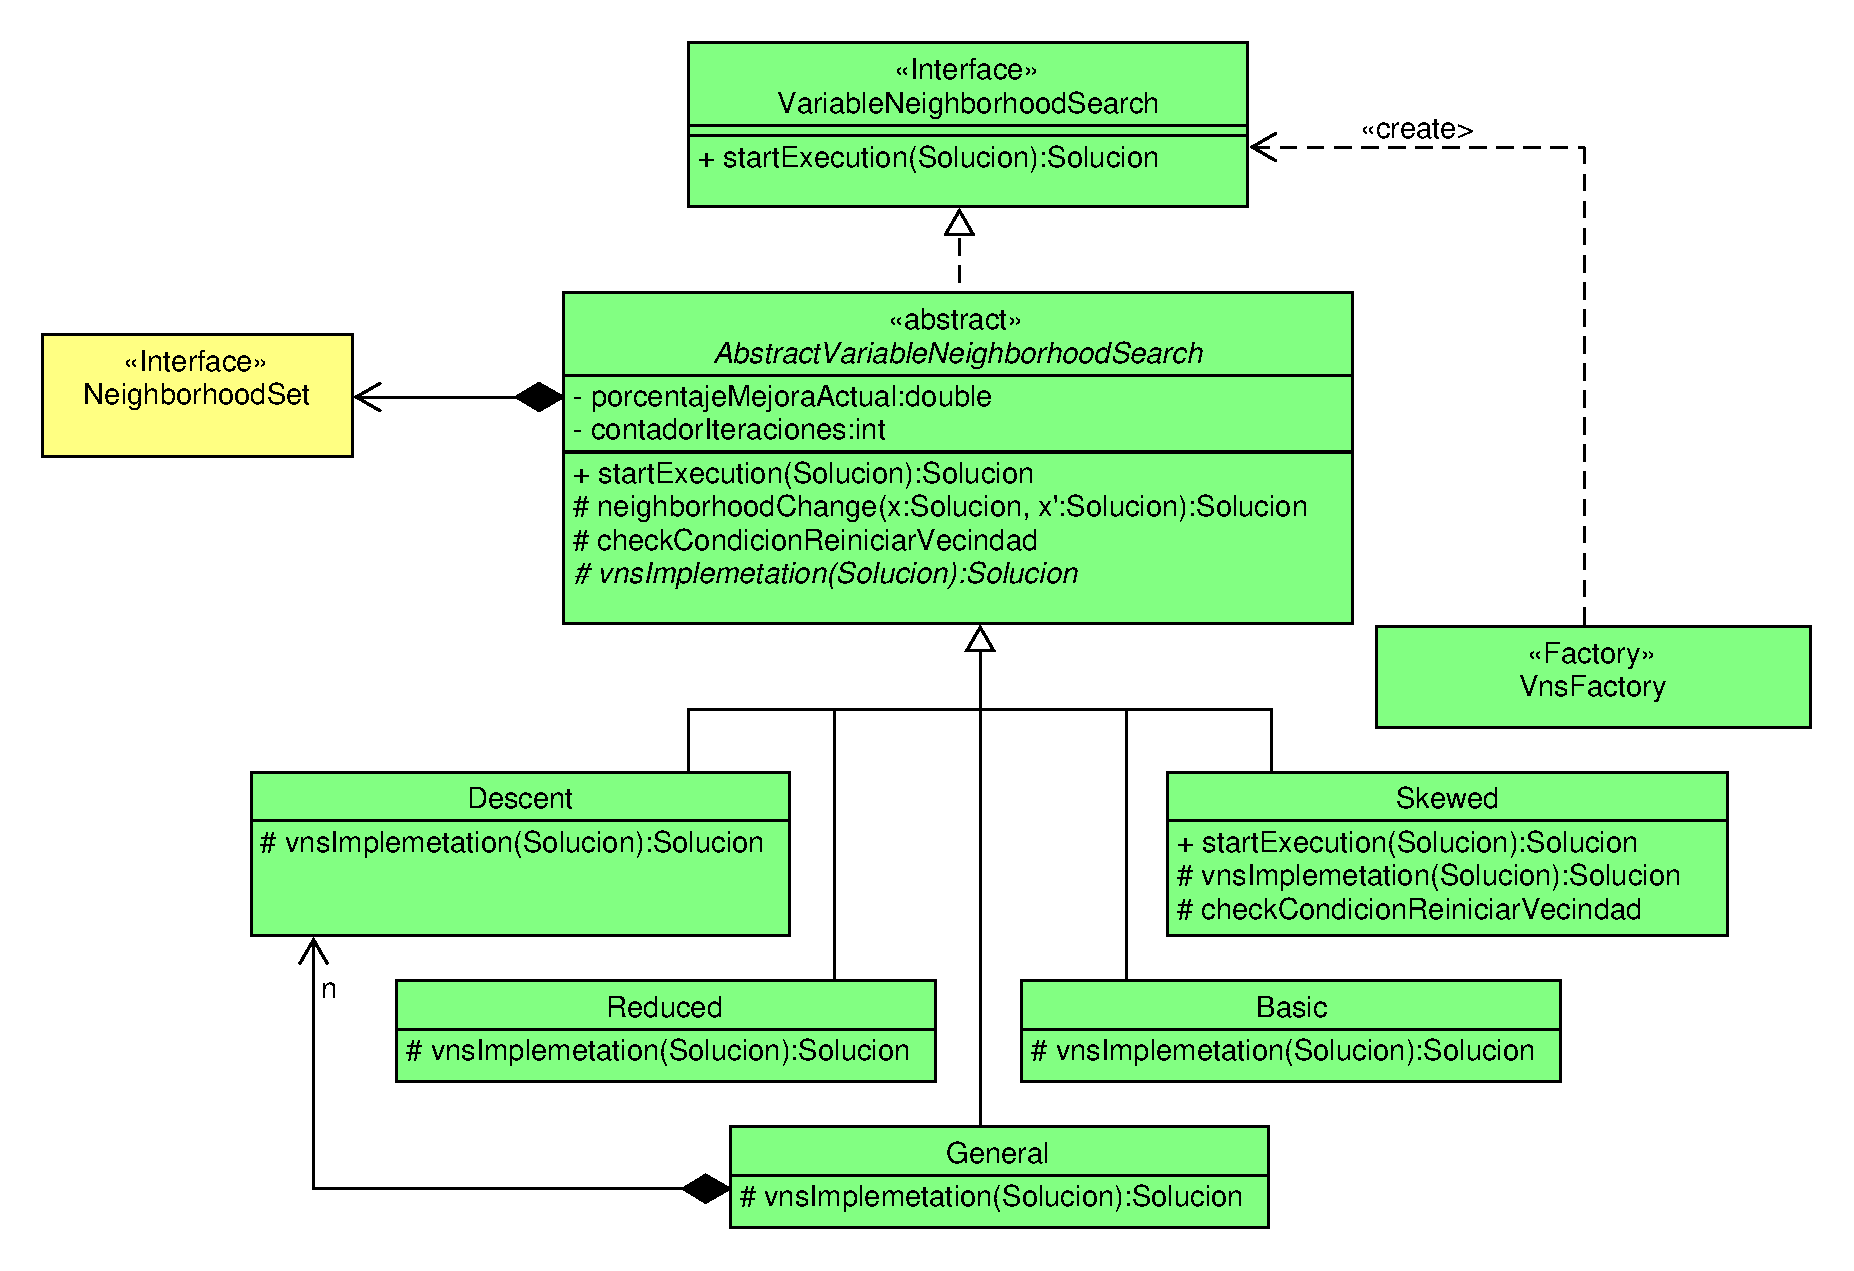
\includegraphics[width=0.9\linewidth]{diagrama-clases-VNS-alt}
	\caption{Esquema del paquete vns (verde)}
	\label{fig:4:diseño:vns}
\end{figure}

\begin{figure}[htbp]
	\centering
	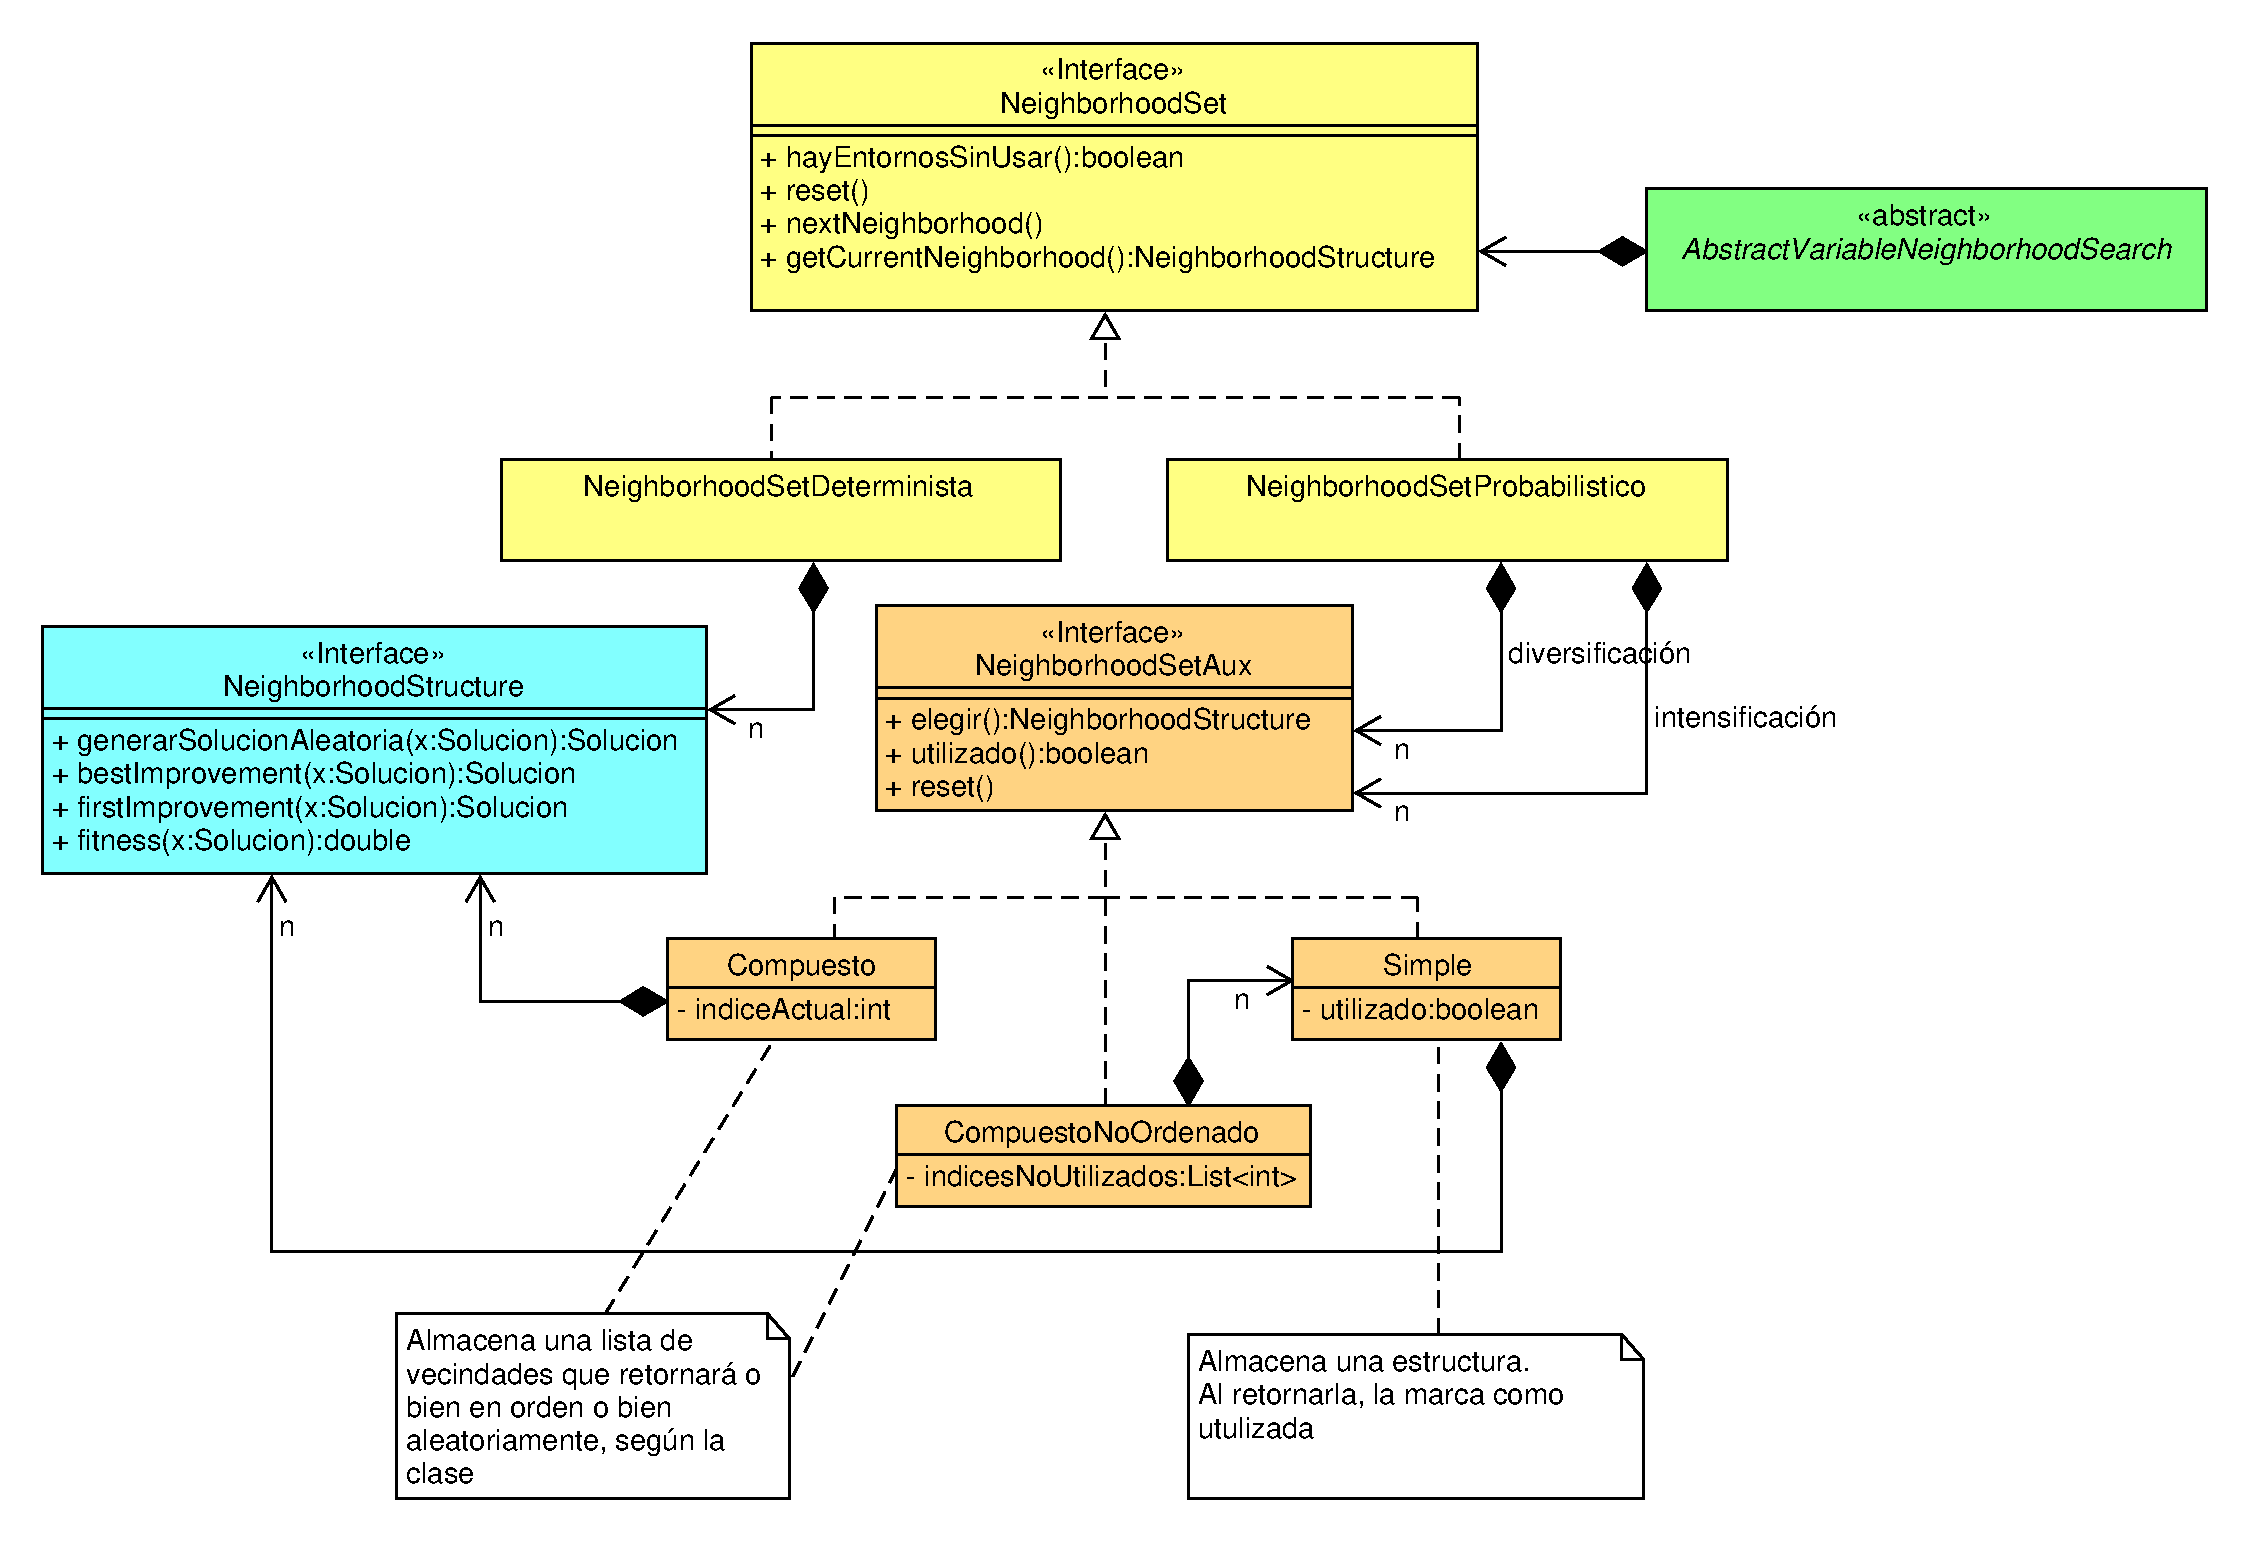
\includegraphics[width=\linewidth]{diagrama-clases-TipoEntornos}
	\caption{Esquema del paquete naturaleza-entornos (amarillo+naranja)}
	\label{fig:4:diseño:tipoEntorno}
\end{figure}

\begin{figure}[htbp]
	\centering
	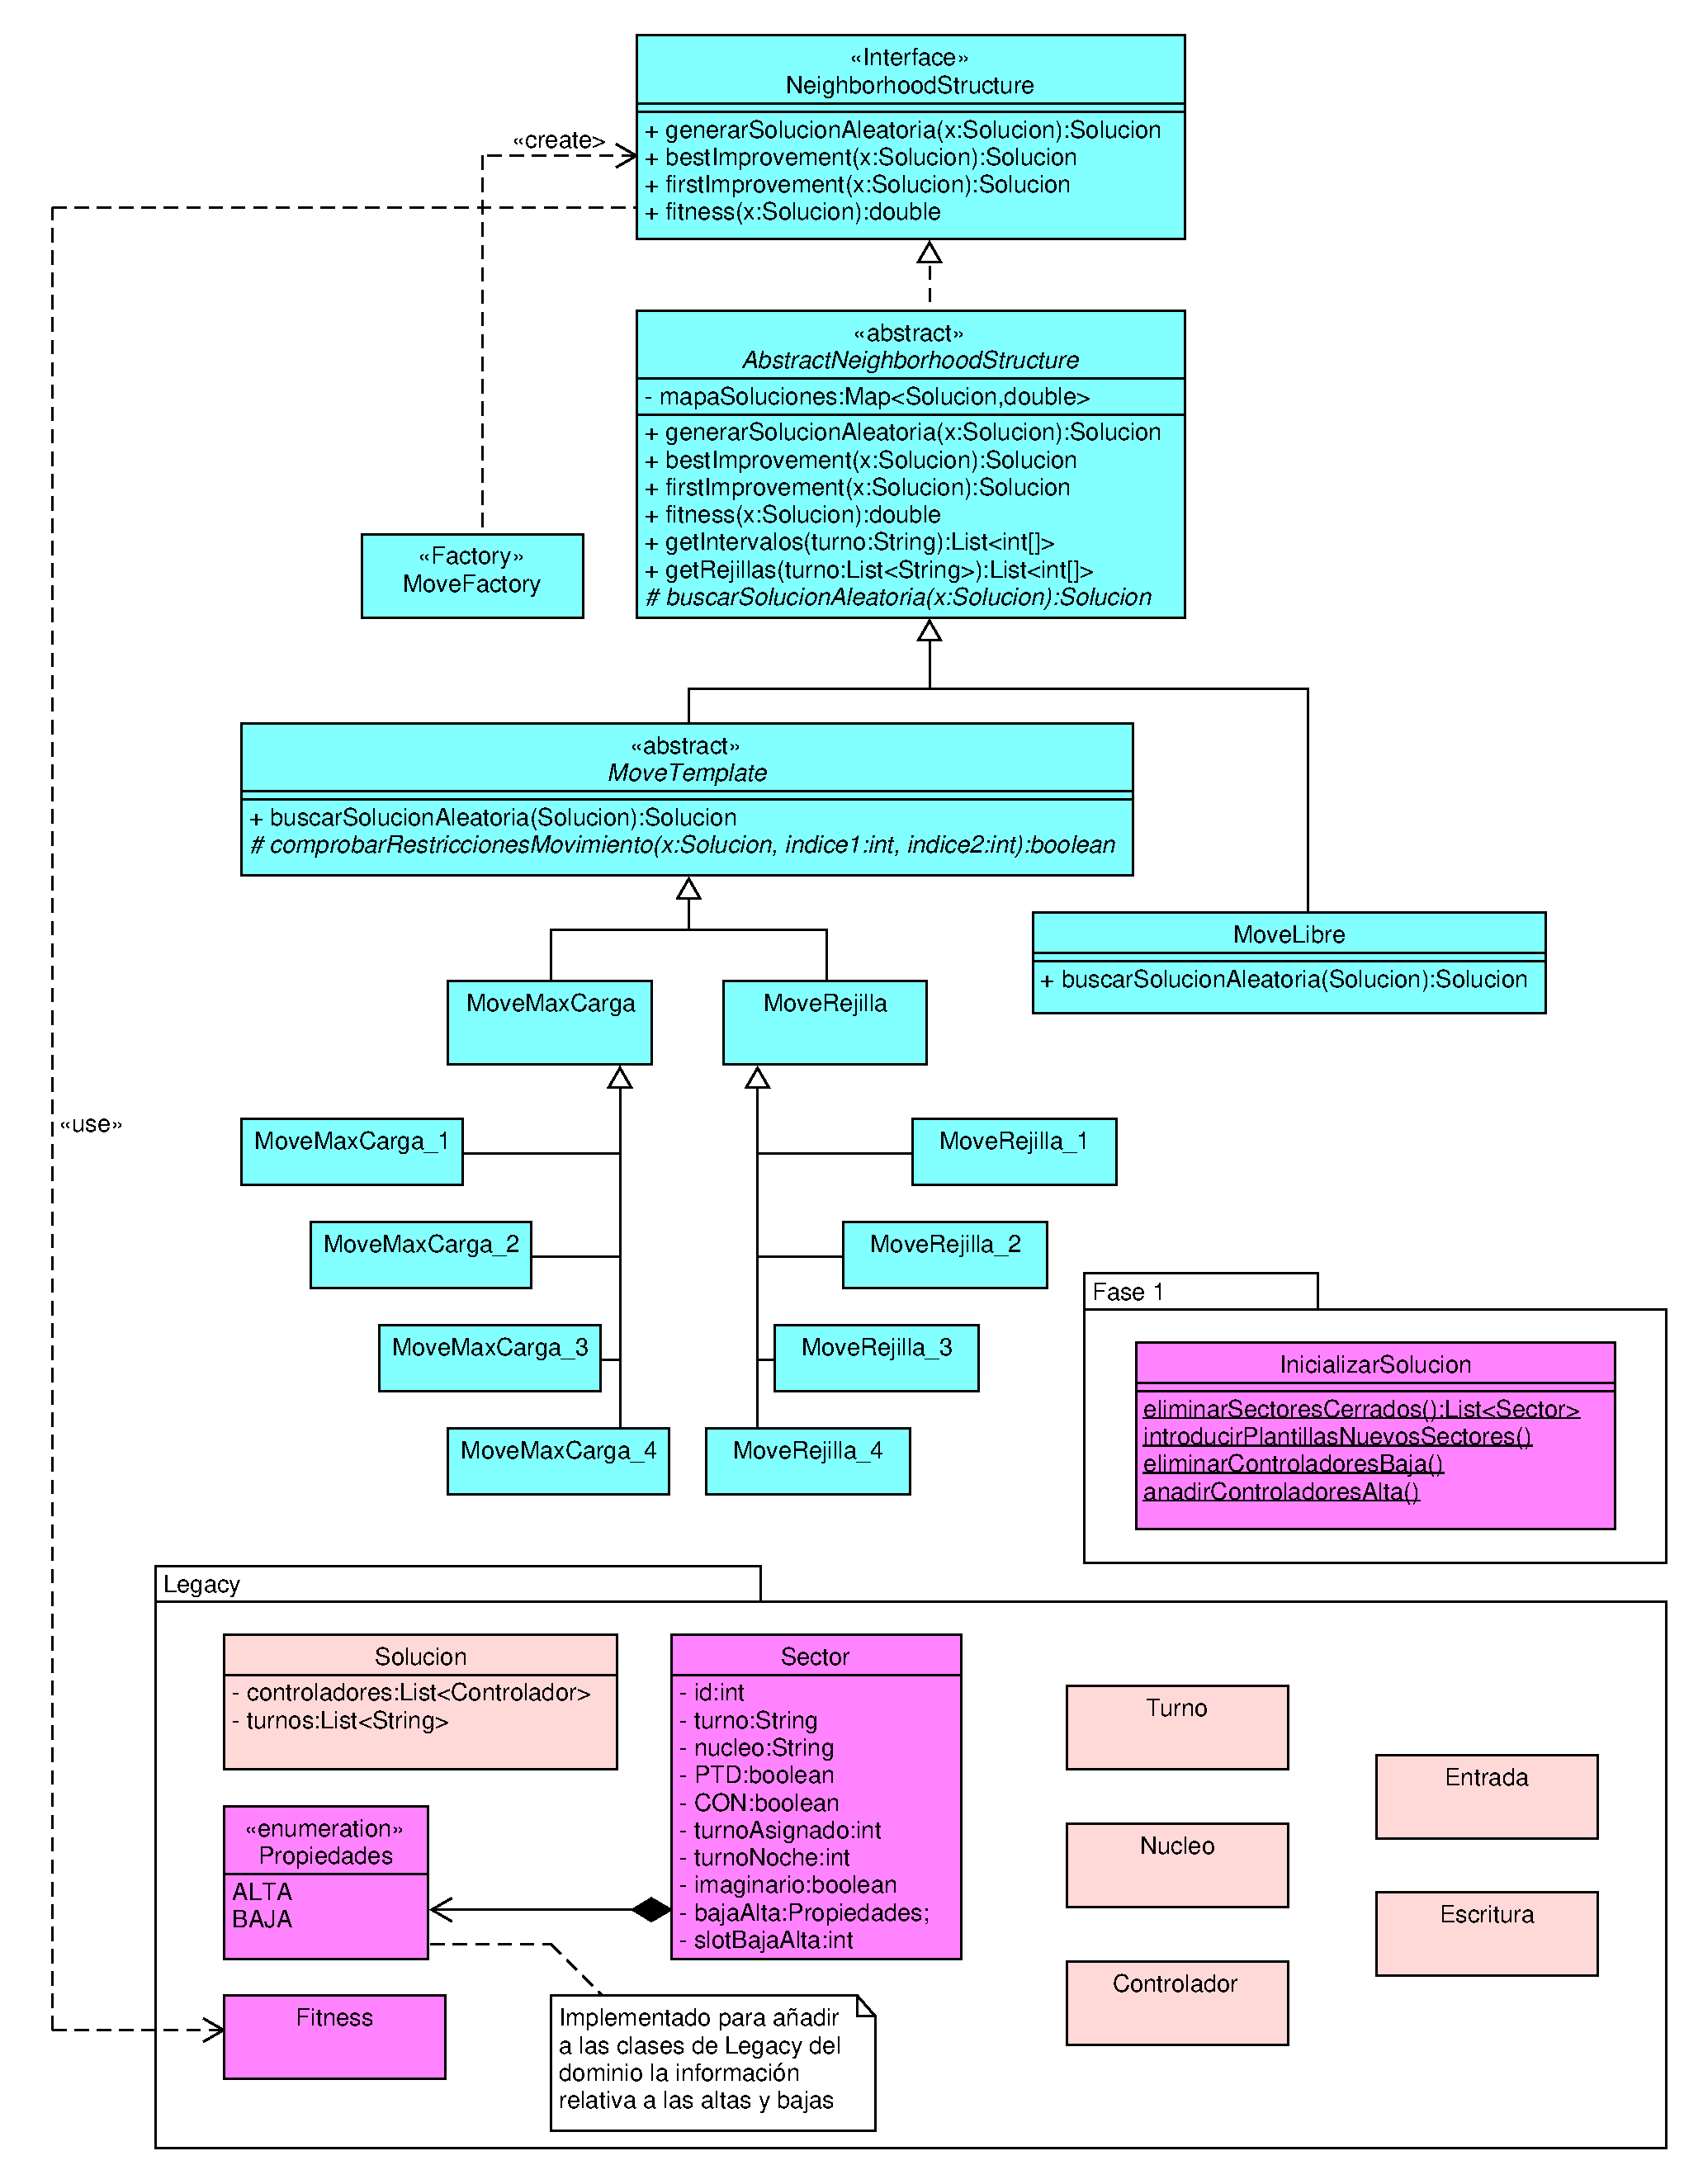
\includegraphics[width=1\linewidth]{diagrama-clases-Vecindades}
	\caption{Esquema del paquete estructuras-entorno (cian)}
	\label{fig:4:diseño:entornos}
\end{figure}


%\subsection{Implementación}
\subsection{Detalles de implementación del sistema}
\label{sec:4:implementacion}

\subsubsection{Herramientas y tecnologías software utilizadas}

Debido a la condicionante del sistema \legacy{}, la mayoría de las decisiones de la tecnología son heredadas. 

La más importante es el lenguaje de programación. Debido a la alta complejidad del sistema y a la eficiencia que éste requiere, el lenguaje de programación preferible hubiese sido C++, pues es orientado a objetos y altamente eficiente. Sin embargo, \legacy{} fue implementado en Java 8, y para poder realizar estudios comparativos de SA frente al VNS, se queriere que ambos estén implementados con la misma tecnología.

El resto de tecnologías que se decidieon utilizar son:

\begin{itemize}
	\item Tello (planificación). Empleado como tablero KANBAN con las tareas a realizar, en proceso y finalizadas.
	\item IntelliJ IDEA (implementación). Entorno de Desarrollo Integrado (IDE) de Java.
	\item Git (implementación). Control de versiones software y compartición de código.
	\item Jupyther Notebook (experimentación). Entorno desarrollado sobre Python empleado para el tratamiento de datos y su representación en forma de gráficas.
	\item Microsoft Office y Umlet (diagramas). Para el diseño previo del sistema así como los diagramas de la memoria.
	\item \TeX{} Studio (documentación).
\end{itemize}

\subsubsection{Frameworks}
Un \textit{framework} es un conjunto de herramientas software empaquetadas para su uso mediante una interfaz definida con un lenguaje de programación, que en este caso es Java 8, como ya se ha mencionado anteriormente.

Los frameworks utilizados han sido:

\begin{itemize}
	\item Maven, para la gestión dinámica de librerias y frameworks. Nos evita tener que gestionar manualmente la inclusión de las librerias/frameworks.
	\item Apache Poi 3.15, Para la escritura de ficheros en formato Microsoft Office Excel (véase el requisito \ref{RIO:formato-excel}).
	\item Apache Commons Lang 3.0, Para el un tratamiento de cadenas de caracteres más eficiente.
	\item The DSI Utilities, dsiutils 2.5.4 (Università degli Studi di Milano). Implementa entre otras cosas, algoritmos de generación de números aleatorios eficientes (véase la \autoref{sec:4:impl:random}).
	\item JUnit 3.5.2, Para las pruebas unitarias (véase la \autoref{sec:4:tests}).
\end{itemize}

\subsubsection{Generador de números aleatorios}
\label{sec:4:impl:random}

Debido a la naturaleza estocástica de la \fasedos{} en cuanto a la generación de soluciones aleatorias, la selección de entornos probabilísticos y la implementación de los movimientos definidos, se ve necesario el uso de alguna librería para muestrear números aleatorios. Java incluye un paquete con una implementación propia, sin embargo, no se trata de uno de los mejores existentes, y debido a que se da uso un gran número de veces, se ha preferido emplear un generador cuyo periodo sea mayor. Se ha optado por emplear el llamado xoroshiro128+ (más inforamción de en \url{http://prng.di.unimi.it/}) con un periodo de $2^{128}$ frente al de java, que es $2^{48}$.

\subsubsection{Detalles del sistema}
\label{sec:4:detalles-sistema}

El sistema fue construido en base al diseño previo, que fue ampliado con la introducción de la funcionalidad relativa a la naturaleza probabilista de los entornos.

Los algoritmos implementados para el VNS ya han sido descritos en detalle en el \autoref{capitulo:3}, sin embargo, la implementación de la naturaleza de los entornos no se ha descrito en profundidad.

La naturaleza de los entornos determinista es simple: unicamente precisa de una estructura de datos de tipo lista y un índice que se vaya incrementando en cada llamada al método \texttt{nextNeighborhood()}. Sin embargo, para la implementación del probabilístico, se requiere de una estructura de datos auxiliar mucho mas compleja.

Se han definido entornos cuyo fundamente es idéntico pero emplea diferentes restricciones de entorno (véase \autoref{paragraph:entornos}). Con este tipo de entornos podemos operar de dos maneras: 
\begin{enumerate}[label={(\Alph*)}]
	\item Considerarlos como sub-entornos y emplearlos en orden o aleatoriamente, es decir, seleccionamos los entornos aleatoriamente, y si el elegido tiene sub-entornos iterarlos en orden.
	\item \label{modelo-no-ordenado} Considerarlos como entornos del mismo nivel, pudiendo ser elegidos con la misma probabilidad que todos los demás.
\end{enumerate}

Los entornos que tienen variantes los llamaremos compuestos, y son únicamente movMaxCarga y movRejilla. Mientras que el resto, movLibre, los llamaremos simples.

En el diagrama de clases de la \autoref{sec:4:diseño} se ha llamado a las clases que implementan el modelo \ref{modelo-no-ordenado} como \texttt{CompuestoNoOrdenado}.

Otros algoritmos tanto nuevos como ampliados se ha visto limitados por la implementación de \legacy{}, en especial la decisión tomada durante el desarrollo del mismo de emplear como representación de los turnos una cadena de texto (String) en lugar de la opción más sencilla de una tupla de elementos. Por ello, la manipulación de los turnos pierde legibilidad de código y gana dificultad de implementación, puesto que las cadenas de turnos son conjuntos sin separadores de 3 letras cada uno (recuérdese la decisión de representación de las soluciones, recopilado en la \autoref{sec:3:representacion-soluciones}) por lo que se deberán recorrer de 3 en 3.

Por otro lado el tratamiento de los Strings es bastante costoso computacionalmente, pues nos obliga a cortar el String y reconstuirlo cada vez que se tenga que modificar. Inicialmente se planteó la posibilidad de tratar de mejorar éste aspecto sustituyendo la forma de representación de los turnos por tuplas, sin embargo, y debido a las decisiones de diseño tomadas durante el desarrollo de \legacy{}, implementar esta mejoría requiere de una gran cantidad de modificaciones y al no ser el aspecto fundamental de la tesis se optó por mantener el formato \legacy{}.

Para el cálculo de probabilidades y simulación de sucesos se muestrea de una distribución aleatoria uniforme entre 0 y 1 $u ~ U[0,1]$ y si la probabilidad p es mayor ($p>u$) se interpreta como que el suceso ocurre, y en caso contrario como si no sucediera. 
La otra alternativa empleada es muestrear uniformemente un entero entre dos números límite. 
Ésto se emplea fundamentalmente para los entornos estocásticos y los las estructuras de entorno (movimientos).

Por otro lado, poder tomar mediciones del rendimiento y desempeño del algoritmo, se ha creado una clase estática extra que permite almacenar en un fichero externo CSV la información requerida (recopilada en el requisito \ref{RIO:salida-csv}).

\subsubsection{Mejorando la eficiencia del sistema}
\label{sec:4:mejorando-eficiencia}

Para mejorar la eficiencia general del sistema, tal y como se propuso en la hipótesis inicial \ref{H3}, se han realizado pequeñas modificaciones para que el sistema consuma menos tiempo en determinadas acciones y que lo pueda emplear en la búsqueda.

Para ello se ha analizado complejidad del sistema en cuanto a tiempo de ejecución de las diferentes partes y se ha obtenido lo dela figura: \NOTE{poner la figura con la eficiencia del sistema por clases. NECESITO EL PC DEL DESPACHO PARA FINALIZAR ESTA SECCIÓN} % TODO!!!

% TODO: . . . 

\subsection{Pruebas}
\label{sec:4:tests}

La mayor parte de las pruebas realizadas al sistema fueron manuales, observando el fichero excel de salida y analizando el comportamiento del algoritmo y detectar así anomalías en él.

Por otro lado, se llevaron a cabo test unitarios para testar la funcionalidad de métodos concretos, sobretodo debido a la dificultad de operar a nivel de carácter (explicado en la \autoref{sec:4:detalles-sistema}).
Por ejemplo, el método \texttt{getIntervalos(turno:String)} que se encarga de cortar el String que representa el turno y seleccionar intervalos de trabajo continuado, retornando los índices de comienzo y fin del intervalo de trabajo continuado. Se ha probado con una cadena de caracteres que comienzan por descanso (``111''), que terminen por descanso, que el descanso esté en el medio y que no haya descanso.

% TODO: ¿hay mas? MIRAR EN EL PC DEL DESPACHO

Respecto a test de integración o carga el sistema no requería de ellos. Sin embargo, y ya fuera del alance definido del proyecto, cuando se produzca el despliegue real de la aplicación en los sistemas aeroportuarios, sí serán requeridas.

\subsection{Despliegue y explotación} 
\label{sec:4:despliegue}

Si bien esta fase software no se ha hecho en profundidad, si se ha preparado una exportación de la aplicación para entregar a los tutores y a \gls{CRIDA} para que estos puedan probar la aplicación por sus propios medios.

La exportación tiene los siguientes ficheros:
\begin{enumerate}
	\item Un fichero ejecutable de tipo \textit{jar}
	\item Un fichero properties con las siguientes propiedades:
	\begin{enumerate}[label*={\arabic*}]
		\item Metaheurística a usar (vns o sa).
		\item Ponderación de cada Fitness.
		\item Tiempo máximo de ejecución.
	\end{enumerate}
	\item Directorio de salida, que contendrá un fichero Excel con la planificación y un fichero txt con el valor de  los fitness desglosados de la solución final.
	\item Directorio de entrada, con subdirectorios de cada Unidad de Control y otro con los diferentes casos definidos
\end{enumerate}

El ejecutable encapsula toda la lógica de negocio del proyecto y permite ejecutarla de forma externa. Hace uso de los demás ficheros externos.

El fichero de propiedades que se emplea en el despliegue es una simplificación de aquel empleado internamente, pues tiene muchos más parámetros que de cara al usuario no son relevantes. El contenido del fichero fue propuesto por los tutores.

